%\newpage
%$ $
%\newpage

\renewcommand{\thesubsection}{\textcolor{red}{\Roman{section}.\arabic{subsection}}}
\renewcommand{\thesubsubsection}{\textcolor{red}{\Roman{section}.\arabic{subsection}.\alph{subsubsection}}}

\setcounter{section}{0}
\sndEnTeteTPUn

\begin{center}
\begin{mdframed}[style=titr, leftmargin=60pt, rightmargin=60pt, innertopmargin=7pt, innerbottommargin=7pt, innerrightmargin=8pt, innerleftmargin=8pt]

\begin{center}
\large{\textbf{TP 1 : Identification d'espèces par tests chimiques}}
\end{center}

\end{mdframed}
\end{center}



\begin{tcolorbox}[colback=blue!5!white,colframe=blue!75!black,title=Objectifs de la séance :]
\begin{itemize}
    \item Respecter les règles de sécurité d’un laboratoire de chimie.
    \item Mettre en œuvre les tests chimiques de présence d’eau, de dihydrogène, de dioxygène et de dioxyde de carbone.

\end{itemize}
\end{tcolorbox}

\begin{tcolorbox}[colback=orange!5!white,colframe=orange!75!black,title= Scénario:]
La majorité des liquides et des gaz mis en jeu lors des expériences de chimie sont incolores. Le chimiste a pourtant besoin de les distinguer : il utilise pour cela des tests chimiques.
\end{tcolorbox}

\section*{Documents mis à disposition}

\begin{doc}{Quelques tests chimiques vus au collège}
    \begin{center}
        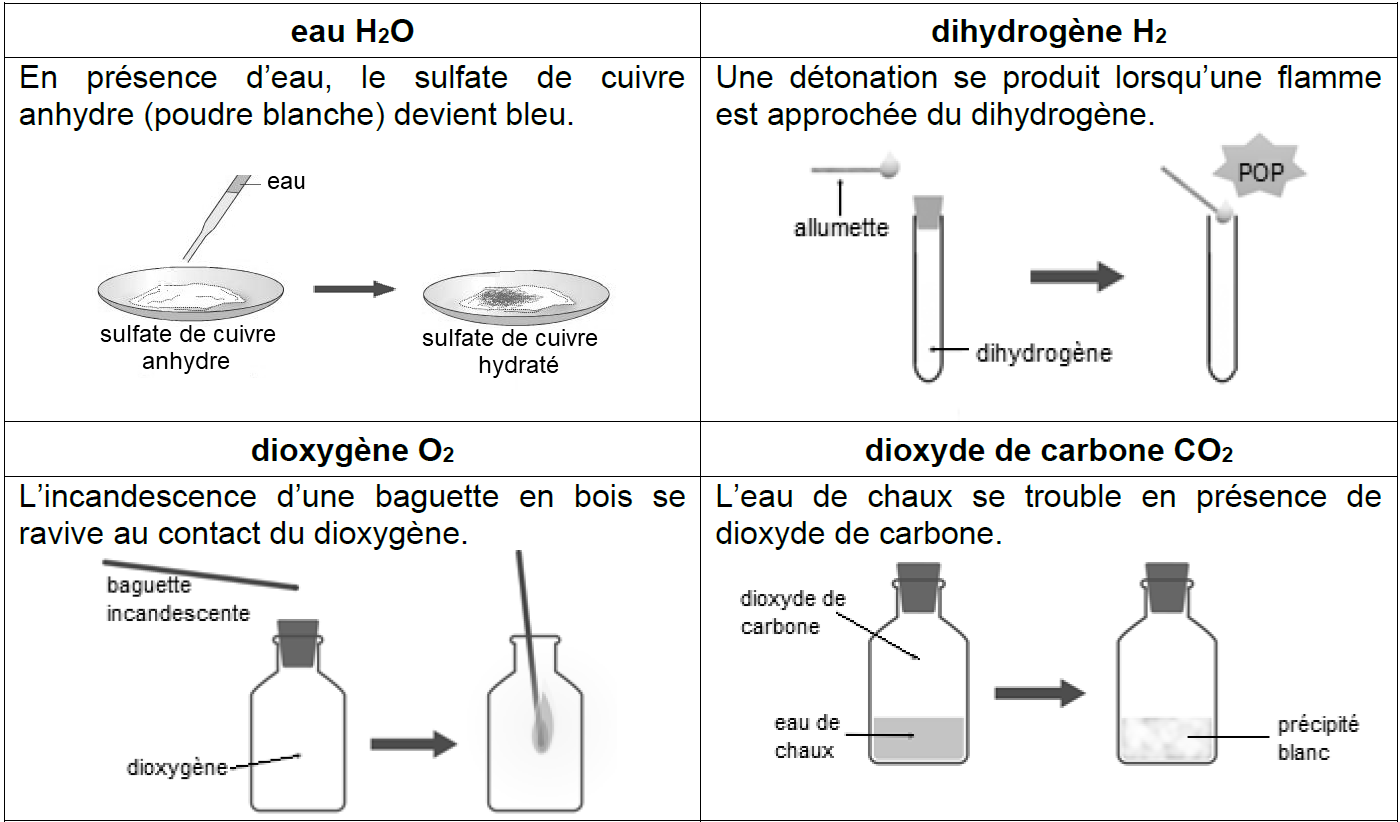
\includegraphics[scale=0.46]{Images/TP1/Tests_chimiques.png}
    \end{center}
\end{doc}

\begin{doc}{Pictogrammes de sécurité des produits utilisés lors du TP}
    \begin{minipage}{0.5\linewidth}
        
        \begin{center}
            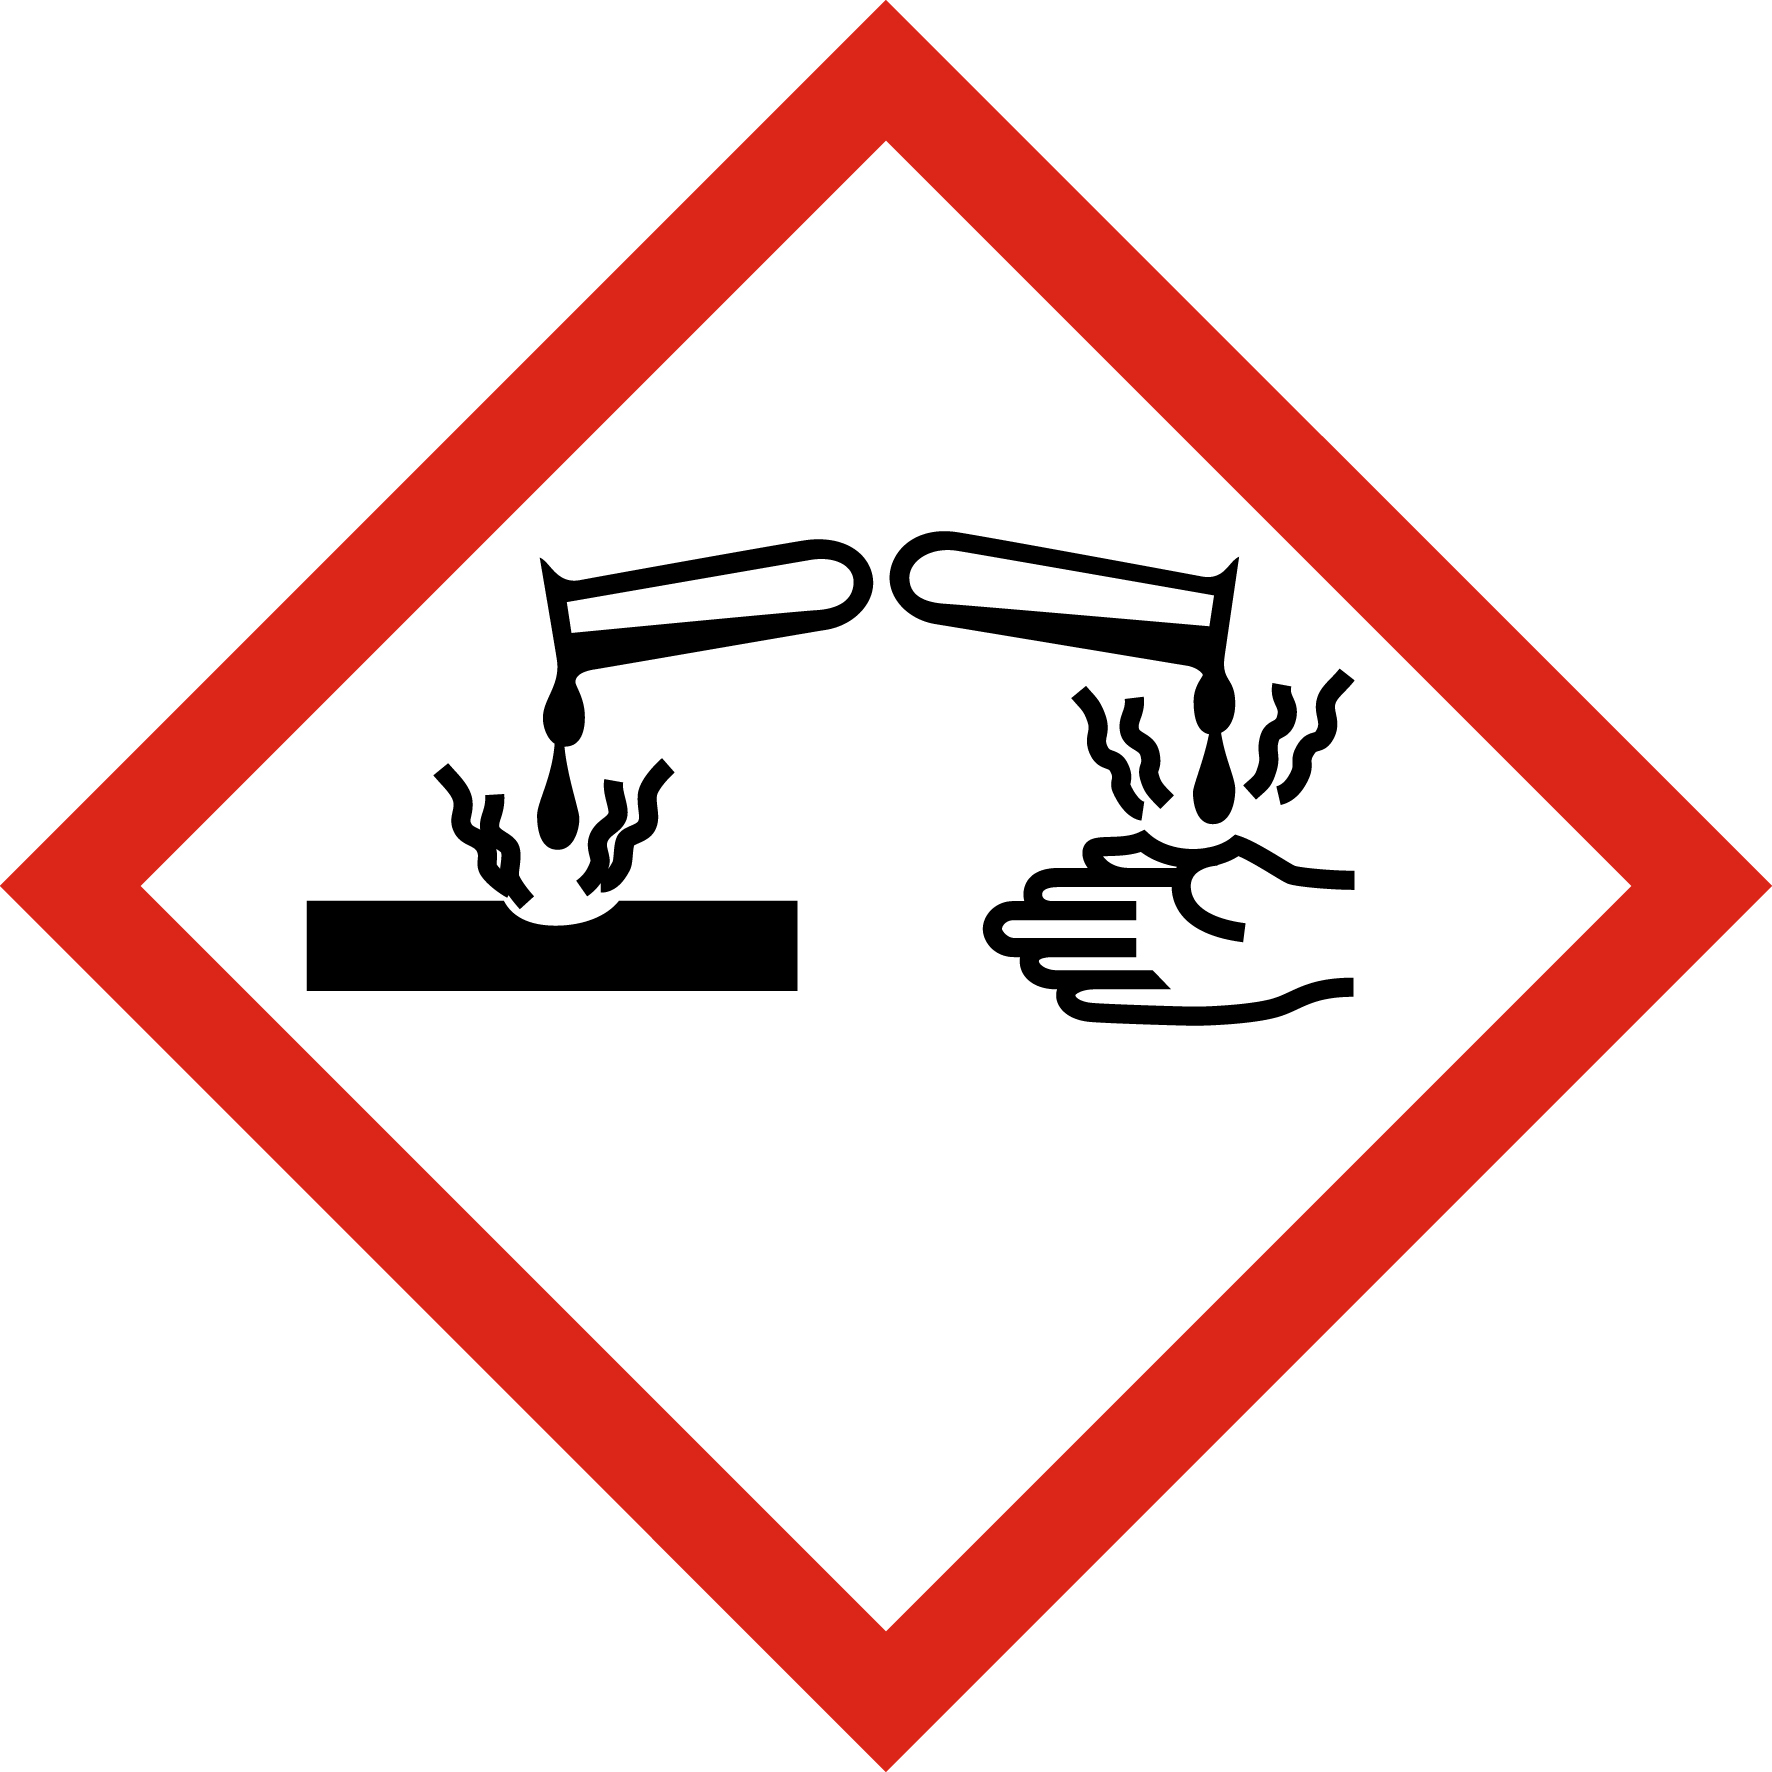
\includegraphics[scale=0.3]{Images/Fiche_Methode1/SGH05_Corrosion.jpg}
        \end{center}
        \begin{itemize}
            \item Solution d'acide chlorhydrique (\chemform{H^+_{(aq)}+Cl^-_{(aq)}})
            \item solution de chlorure de fer III (\chemform{Fe^{3+}_{(aq)}+3Cl^-_{(aq)}})
            \item eau oxygénée \chemform{H_2O_2}
        \end{itemize}
        
    \end{minipage}
    \begin{minipage}{0.5\linewidth}\vspace{-1.8cm}
    \begin{center}
        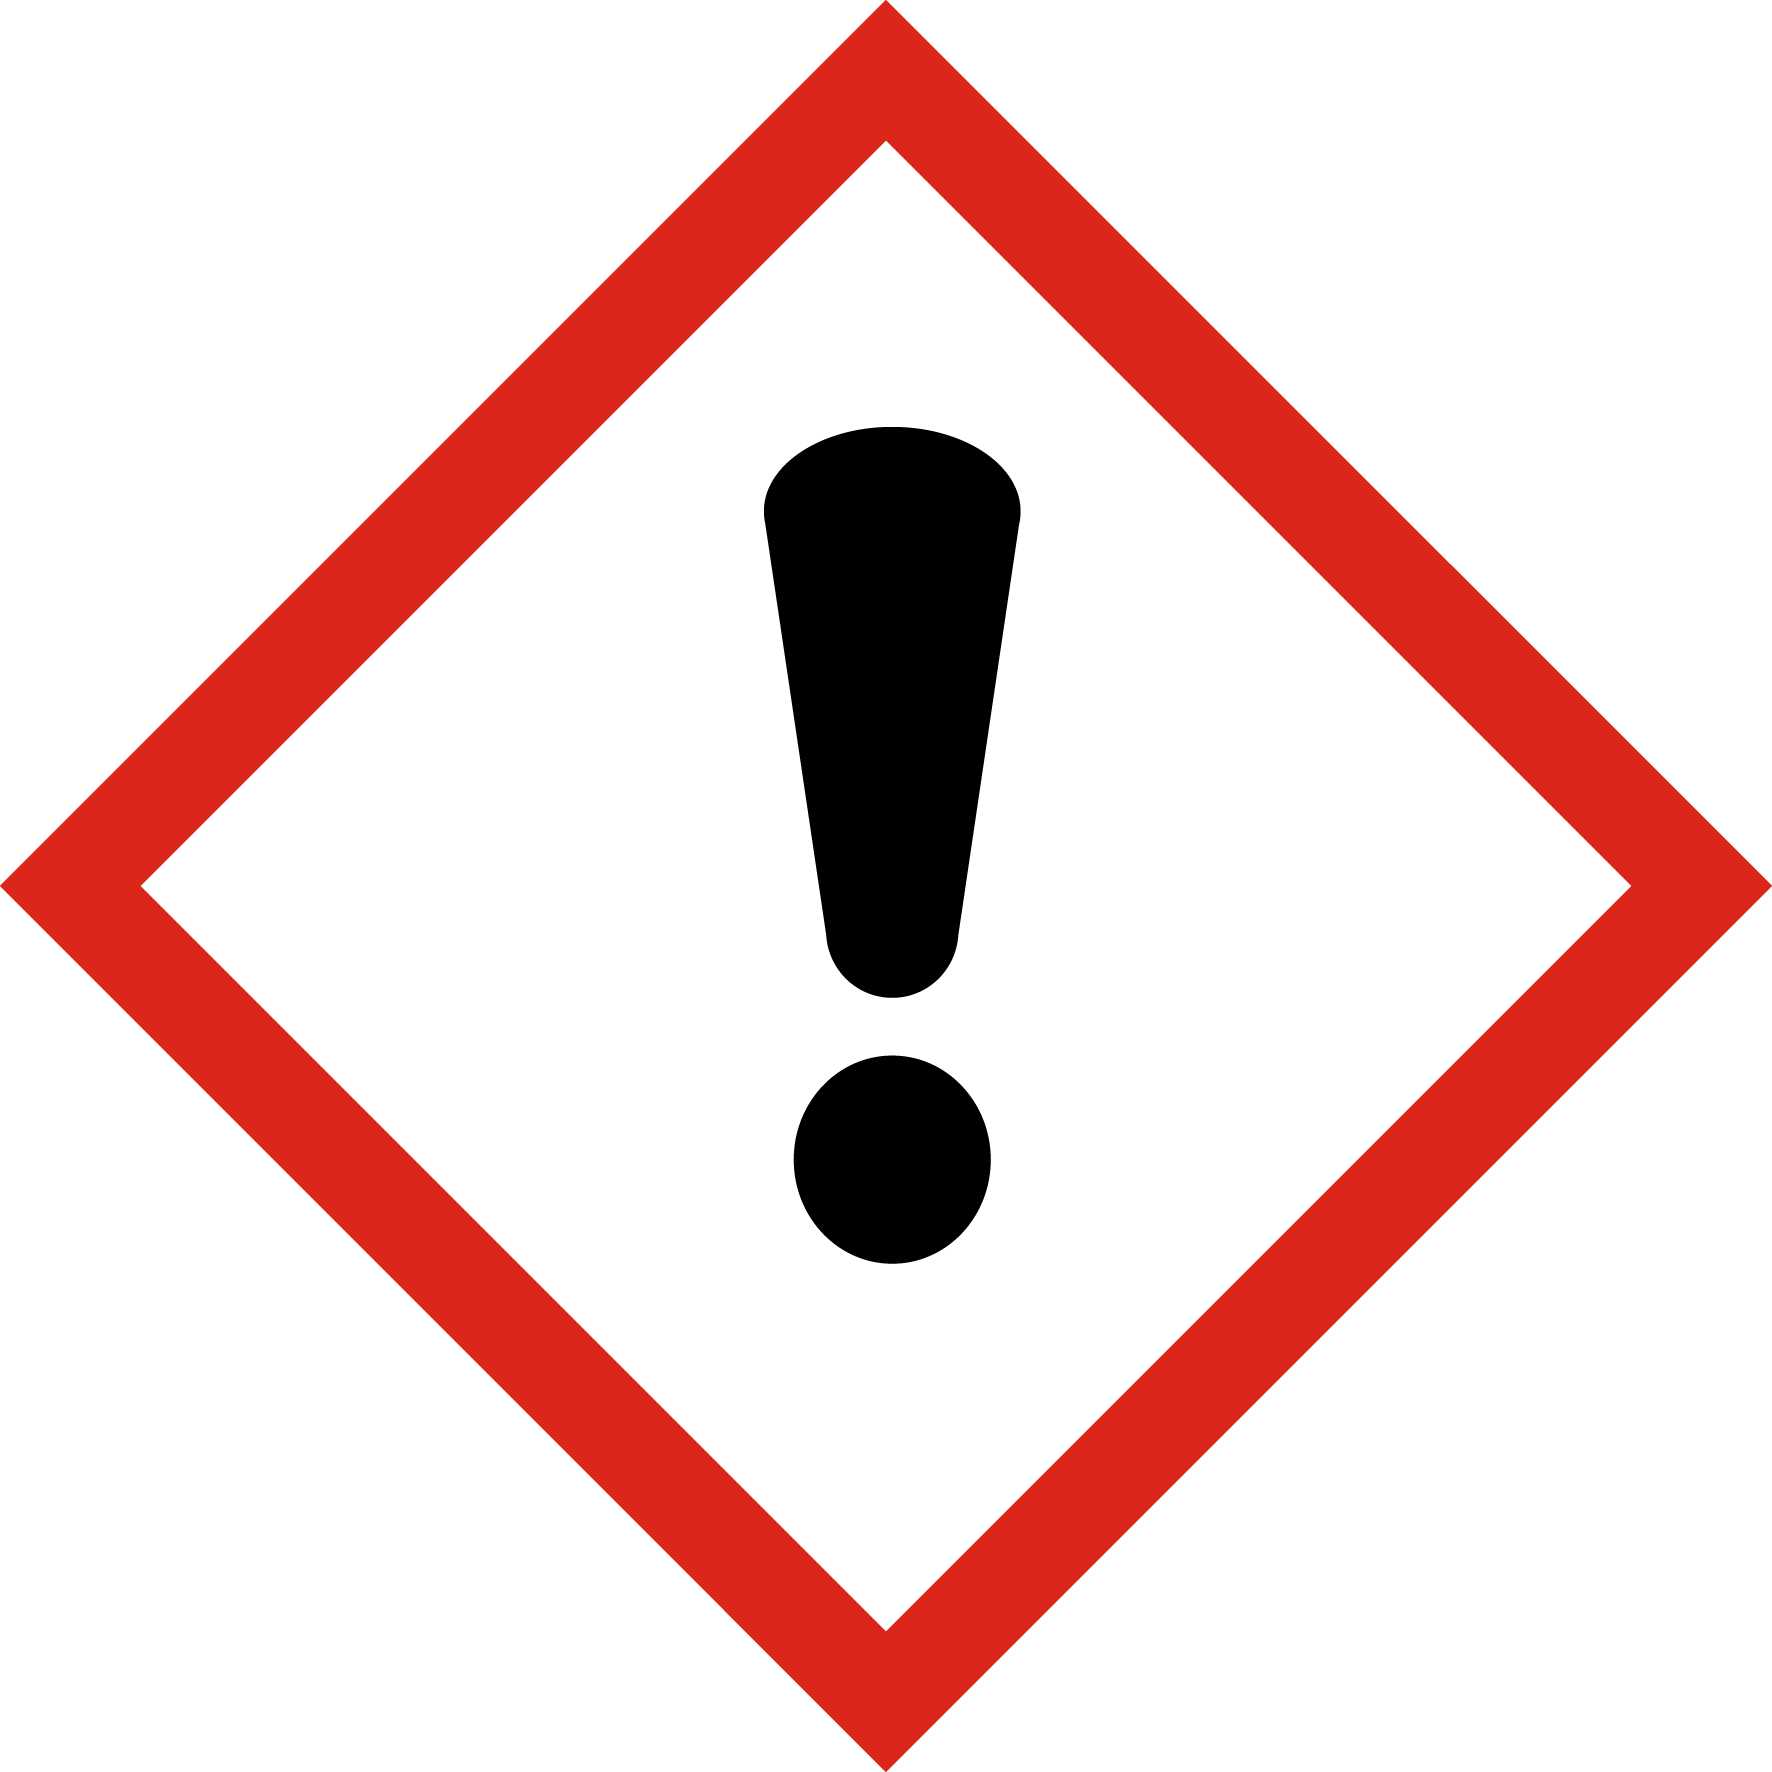
\includegraphics[scale=0.3]{Images/Fiche_Methode1/SGH07_PointExclamation.jpg}
    \end{center}
    \begin{itemize}
            \item eau de chaux (\chemform{Ca^{2+}_{(aq)}+HO^-_{(aq)}})
            \item sulfate de cuivre anhydride \chemform{CuSO_4(s)}
    \end{itemize}
    \end{minipage}
    \vspace{1cm}
    
    \begin{large}
        \ding{52}
    \end{large}Pour s'approprier les pictogrammes de sécurité : \url{https://learningapps.org/display?v=pz0yp6isn23} 
\end{doc}

\begin{doc}{Protocoles expérimentaux}
\begin{minipage}{\linewidth}
\begin{center}
    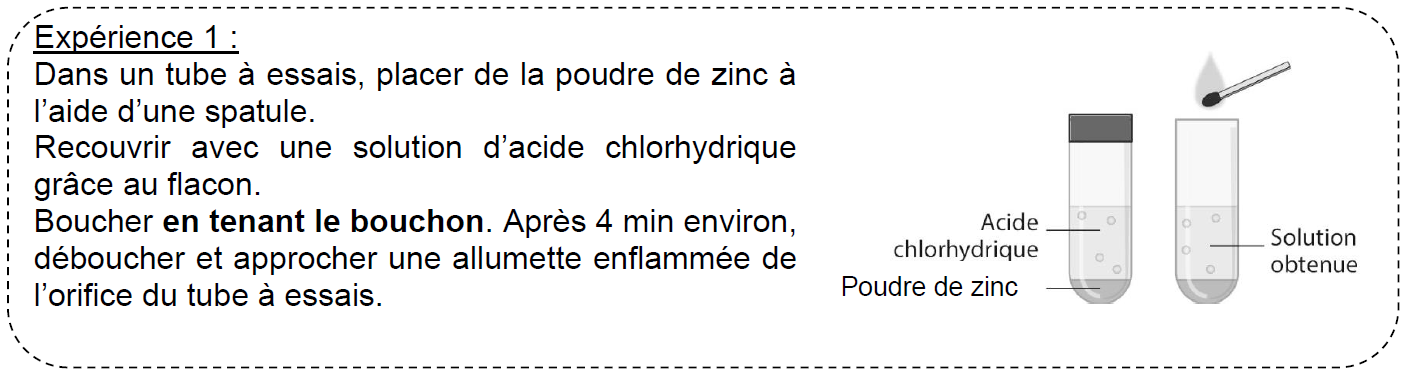
\includegraphics[scale=0.46]{Images/TP1/Exp_H2.png}
\end{center}
\end{minipage}
\begin{minipage}{\linewidth}
\begin{center}
    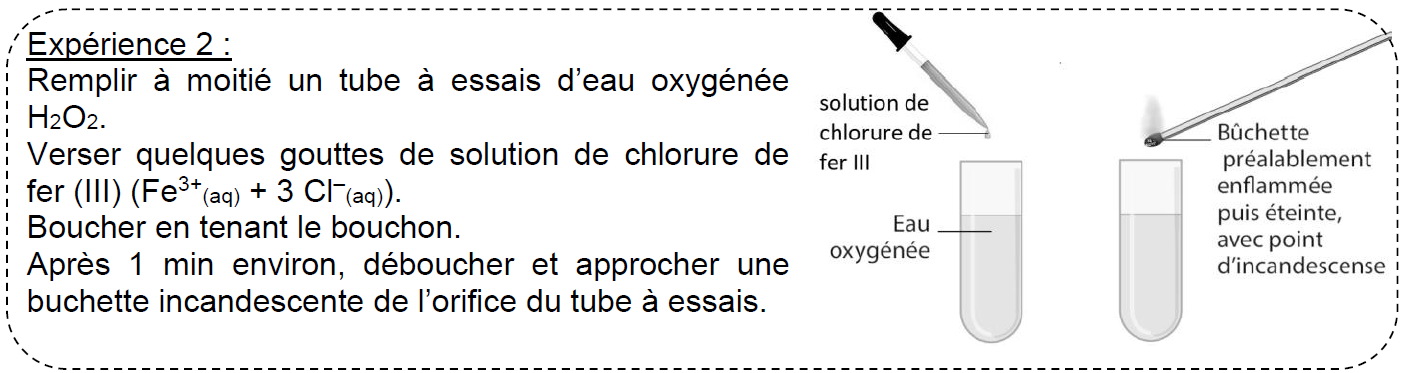
\includegraphics[scale=0.46]{Images/TP1/Exp_O2.png}
\end{center}
\end{minipage}
\begin{minipage}{\linewidth}
\begin{center}
    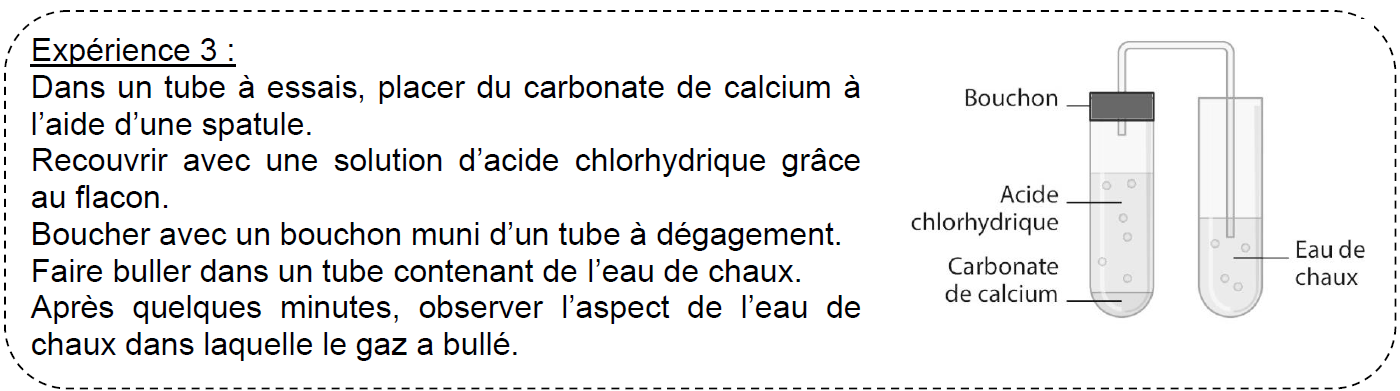
\includegraphics[scale=0.46]{Images/TP1/Exp_CO2.png}
\end{center}
\end{minipage}
\end{doc}

\begin{mdframed}[style=autreexo]
\textbf{\bsc{Liste du matériel}}
\begin{itemize}
    \item un flacon contenant de la poudre de zinc ;
    \item un flacon contenant une solution d’acide chlorhydrique ;
    \item un flacon contenant de l’eau oxygénée \chemform{H_2O_2};
    \item un flacon contenant une solution de chlorure de fer III ;
    \item un flacon contenant du carbonate de calcium en poudre ;
    \item une pissette d'éthanol à 95\% ;
    \item une solution de glycérol ;
    \item une spatule ;
    \item une boite d’allumettes ;
    \item une bûchette en bois ;
    \item des tubes à essais et leur support ;
    \item des bouchons pour tubes à essais ;
    \item un tube à dégagement et un bouchon pour tube à essais adapté ;
    \item une coupelle ;
    \item des béchers ;
    \item des pipettes simples ;
	\item des gants et des lunettes de protection.
 
\end{itemize}
\end{mdframed}

\newpage

\begin{Large}
    \textbf{\textcolor{red}{Travail à effectuer :}}
\end{Large}
\\
\begin{enumerate}
    \item Allumer votre ordinateur. Aller sur le site \url{https://learningapps.org/display?v=pz0yp6isn23} et effectuer l'activité.
    \item À l’aide du document 2, expliquer pourquoi il sera obligatoire de porter des gants, en plus de la blouse et des lunettes de protection, tout au long de l’activité.
    \item Réaliser les trois expériences du document 3 et noter vos observations expérimentales.
    \item À l’aide du document 1, identifier pour chacune des expériences du document 3 le gaz libéré.
    \item Compléter le tableau du document de cours avec vos observations
    \item On dispose de deux solutions : une d'éthanol commerciale et une de glycérol. Proposer un protocole permettant de déterminer si ces solutions contiennent de l'eau.
    \item Appeler le professeur pour valider ce protocole.
    \item Mettre en \oe uvre le protocole et noter vos observations expérimentales.
    \item La solution d'éthanol est-elle pure ? Que veut dire \og Solution d'éthanol à 95\% \fg ?
\end{enumerate}

\textit{Bonus pour les plus rapides : calculer la masse d'éthanol contenue dans la bouteille suivante : }

\begin{minipage}{0.5\textwidth}
\centering
    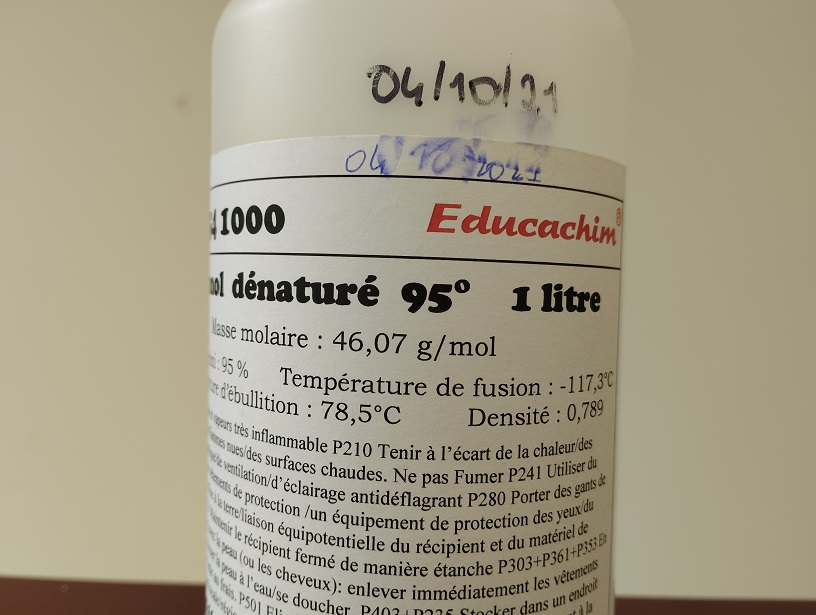
\includegraphics[scale=0.3]{Images/TP1/Bouteille_ethanol.jpg}
\end{minipage}
\begin{minipage}{0.5\textwidth}
\centering
    
\includegraphics[scale=0.3]{Images/TP1/qrcode_picto.png}
    \\
    QR-code pour les pictogrammes de sécurité.
\end{minipage}

